\chapter{Resultados e discussão}

O presente capítulo apresenta e discute os resultados obtidos a partir da aplicação da metodologia \textit{Methontology} \cite{fernandez1997methontology} no desenvolvimento da ontologia proposta para o MPO \cite{vieira2022thesis} (OntoMPO). Diferentemente do capítulo anterior, que teve como foco a descrição metodológica das etapas adotadas, este capítulo concentra-se nos artefatos produzidos, nas decisões de modelagem realizadas e na análise crítica dos resultados alcançados em cada etapa do processo ontológico.

Em conformidade com a \textit{Methontology} \cite{fernandez1997methontology}, os resultados são organizados segundo suas principais etapas. Cada seção descreve os procedimentos adotados, os artefatos intermediários gerados e a forma como o conhecimento do domínio dos observatórios de projetos, fundamentado no MPO \cite{vieira2022thesis}, foi progressivamente estruturado e refinado.

Os resultados desta pesquisa devem ser compreendidos à luz do objetivo central do trabalho, que consiste na proposição e formalização de uma ontologia de domínio para observatórios de projetos. Assim, a avaliação conduzida não visa comprovar o desempenho da ontologia em ambientes operacionais completos, mas analisar sua adequação conceitual, consistência lógica, aderência ao modelo conceitual MPO \cite{vieira2022thesis} e potencial de reutilização e extensão.

\subsection{Questões de competência}

As questões de competência (QCs) representam perguntas que a ontologia deve ser capaz de responder e são utilizadas como mecanismo de definição de requisitos e de validação do modelo ontológico. Conforme estabelecido pela metodologia Methontology \cite{fernandez1997methontology}, essas questões orientam o desenvolvimento da ontologia, permitindo verificar se o modelo é capaz de representar adequadamente os conceitos e relações relevantes do domínio.

No contexto deste trabalho, as questões de competência foram definidas com base no domínio dos observatórios de projetos descrito pelo MPO \cite{vieira2022thesis}. Essas questões procuram refletir aspectos estruturais e relacionais do modelo, incluindo a organização hierárquica dos conceitos e as interações entre as diferentes camadas do domínio. O Quadro \ref{quadro:qcs} apresenta o conjunto de questões de competência consideradas no desenvolvimento da ontologia.

\begin{table}[H]
\centering
\caption{Questões de competência da ontologia}
\label{quadro:qcs}

\begin{tabular}{p{2cm} p{12cm}}
\hline
\textbf{QC} & \textbf{Questão de Competência} \\
\hline
QC1 & Como os conceitos da ontologia estão organizados hierarquicamente? \\
QC2 & Como os conceitos associados à camada de estruturas são representados na ontologia? \\
QC3 & Como os conceitos associados à camada de processos são representados na ontologia? \\
QC4 & Como os conceitos associados à camada de agentes são representados na ontologia? \\
QC5 & Quais são as relações existentes entre estruturas, processos e agentes? \\
\hline
\end{tabular}

Fonte: Próprio autor.
\end{table}

\section{Conceitualização}

Essa etapa foi realizada em conformidade com a \textit{Methontology} \cite{fernandez1997methontology}, a qual estabelece a conceitualização como uma fase fundamental do processo de desenvolvimento ontológico, responsável por organizar o conhecimento do domínio de forma independente de formalismos computacionais. No contexto desta pesquisa, a conceitualização da OntoMPO teve como objetivo sistematizar o conhecimento proveniente do MPO \cite{vieira2022thesis}, resultando na identificação e organização dos conceitos associados às camadas de Estruturas, Processos e Agentes \cite{vieira2022thesis}. Para atender a esse objetivo, foram produzidos diversos artefatos conceituais, incluindo o glossário de termos, árvores de classificação de conceitos, dicionários de dados, tabelas de atributos, instâncias, constantes, fórmulas e regras \cite{fernandez1997methontology}, bem como artefatos voltados à modelagem de ações e relações, tais como o dicionário de verbos e a tabela de condições \cite{fernandez1997methontology}.

Visando manter o foco do capítulo na análise e discussão dos resultados, os artefatos completos gerados nesta etapa são apresentados de forma detalhada no Apêndice~\ref{ap:conceitualizacao} deste trabalho. A seguir, é apresentada uma visão geral dos resultados obtidos na etapa de conceitualização, com a indicação dos principais elementos produzidos.

\begin{itemize}
    \item \textbf{Glossário de termos}: 53 termos.
    \item \textbf{Árvore de classificação de conceitos}:
    \begin{itemize}
        \item \textbf{Dicionário de dados}: 17 conceitos;
        \item \textbf{Atributos de instância}: 41 atributos;
        \item \textbf{Atributos de classe}: 40 atributos;
        \item \textbf{Tabelas de constantes}: 20 constantes;
        \item \textbf{Tabelas de instâncias}: 53 instâncias;
    \end{itemize}
    \item \textbf{Diagrama de verbos}:
    \begin{itemize}
        \item \textbf{Dicionário de verbos}: 15 verbos;
        \item \textbf{Tabela de condições}: 67 condições;
    \end{itemize}
    \item \textbf{Tabela de fórmulas}: 55 fórmulas;
\end{itemize}

\begin{figure}[H]
    \centering
    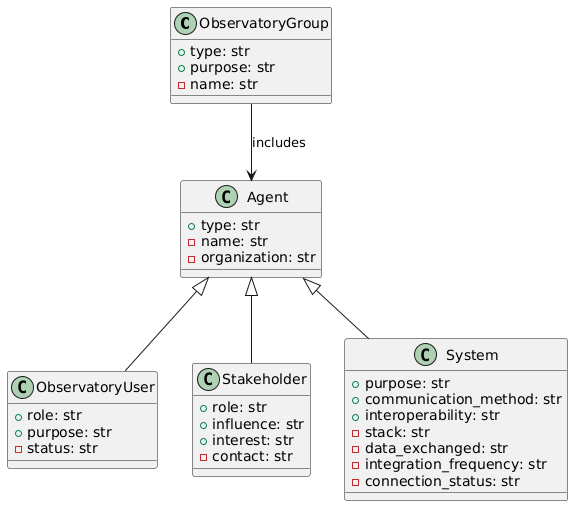
\includegraphics[width=0.75\linewidth]{imagens/mpo_agents_classification_tree.png}
    \caption{Árvore de classificação de conceitos da camada Agentes do MPO. Fonte: Próprio autor.}
    \label{fig:mpo_class_tree}
\end{figure}

\begin{figure}[H]
    \centering
    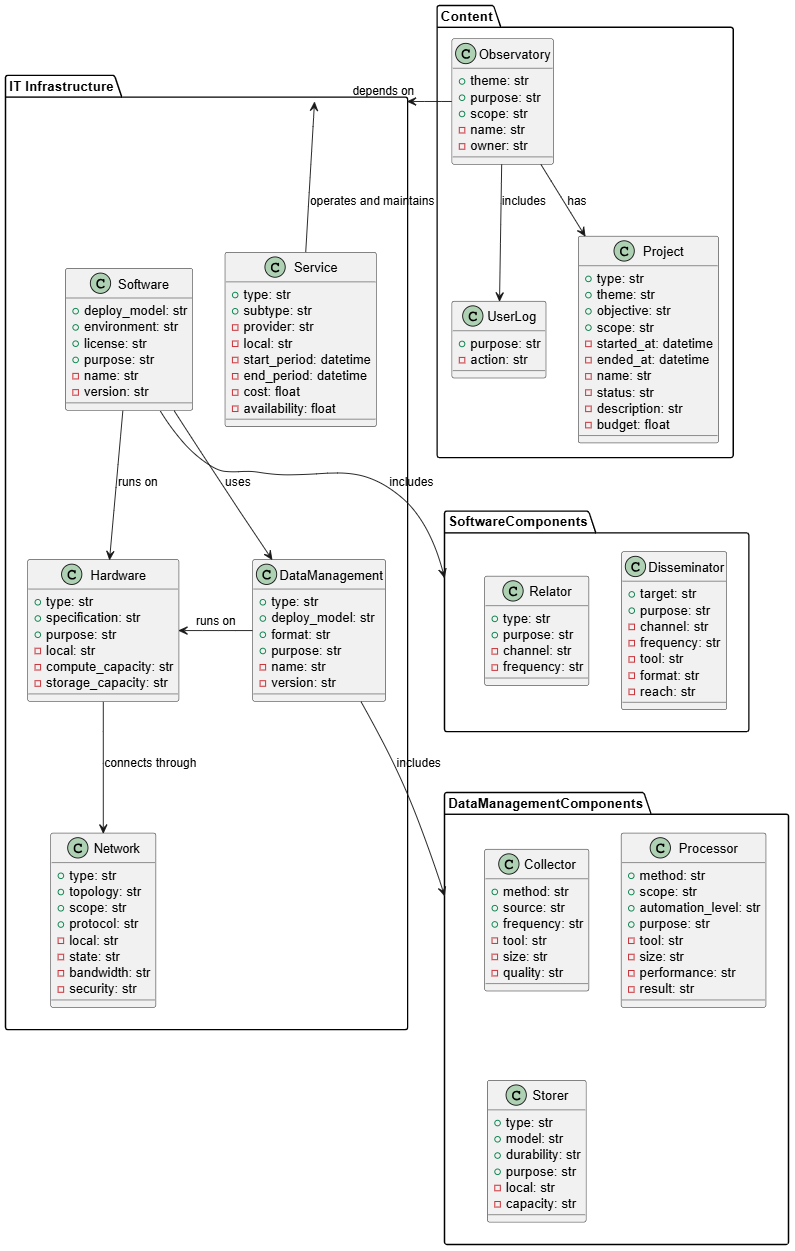
\includegraphics[width=1\linewidth]{imagens/mpo_structures_classification_tree.png}
    \caption{Árvore de classificação de conceitos da camada estruturas do MPO. Fonte: Próprio autor.}
    \label{fig:mpo_class_tree}
\end{figure}

\section{Formalização e Integração}
A etapa de formalização e integração corresponde à fase em que os resultados obtidos na conceitualização são transformados em uma representação ontológica formal, dotada de semântica rigorosa e fundamentação ontológica \cite{fernandez1997methontology}. Conforme estabelecido pela \textit{Methontology} \cite{fernandez1997methontology}, essa etapa visa garantir consistência conceitual, reduzir ambiguidades semânticas e promover a integração da ontologia desenvolvida a modelos ontológicos consolidados.

No contexto desta pesquisa, a formalização da OntoMPO foi realizada por meio da linguagem OntoUML \cite{ontouml_readthedocs}, a qual é fundamentada na UFO \cite{guizzardi2008grounding}. A adoção da OntoUML \cite{ontouml_readthedocs} possibilitou a representação explícita dos conceitos do domínio por meio de estereótipos ontologicamente fundamentados, tais como \textit{kind}, \textit{subkind}, \textit{role} e \textit{phase} \cite{ontouml_readthedocs}, assegurando coerência semântica e rigor ontológico. Nesse contexto, a integração da OntoMPO ocorre de forma intrínseca ao próprio processo de formalização, uma vez que o uso da OntoUML \cite{ontouml_readthedocs} implica o alinhamento automático dos conceitos modelados às categorias ontológicas da UFO \cite{guizzardi2008grounding}. Como resultado, a ontologia proposta herda princípios ontológicos amplamente aceitos, promovendo padronização conceitual, interoperabilidade semântica e reuso de fundamentos ontológicos, sem a necessidade de mapeamentos explícitos com ontologias externas de domínio.

O MPO \cite{vieira2022thesis} é estruturado em três camadas principais, cada uma composta por suas respectivas subcamadas. Os diagramas desenvolvidos em OntoUML \cite{ontouml_readthedocs} adotam uma abordagem baseada em múltiplas visões, nas quais cada camada é representada por diferentes diagramas, alguns com uma perspectiva mais geral e outros com uma perspectiva mais específica. Vale ressaltar que também são utilizados diagramas que retratam relações entre diferentes camadas, bem como diagramas que detalham as relações internas entre os próprios elementos de uma mesma camada. Essa estratégia de modelagem permite que os diagramas se complementem, favorecendo tanto a compreensão global do modelo quanto o detalhamento dos aspectos particulares do domínio.

O diagrama a seguir tem como objetivo representar a infraestrutura que sustenta o funcionamento do Observatório de Projetos. Nele são modelados os elementos pertencentes à subcamada de Infraestrutura de TI do MPO \cite{vieira2022thesis}, bem como sua associação com o elemento Observatório, integrante da subcamada Conteúdos. Todos esses elementos são representados no contexto da camada Estruturas do MPO \cite{vieira2022thesis}, evidenciando as relações e dependências que compõem a base estrutural do observatório.

\begin{figure}[H]
    \centering
    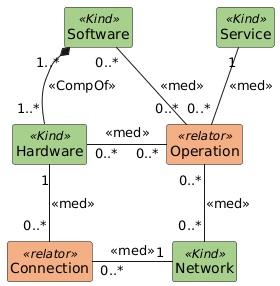
\includegraphics[width=0.6\linewidth]{imagens/mpo_structures_observatory_infra_formalization.png}
    \caption{Formalization of an observatory's infrastructure according to the MPO. Source: Author's own work.}
    \label{fig:mpo_class_tree}
\end{figure}

As classes \textit{Software}, \textit{Hardware}, \textit{Network} e \textit{Service} são modeladas como \textit{kinds} \cite{ontouml_readthedocs}, representando entidades ontologicamente rígidas do domínio. O \textit{ProjectObservatory} é modelado como um \textit{subkind} \cite{ontouml_readthedocs} de \textit{Software}, indicando uma especialização desse tipo. As classes \textit{Connection} e \textit{Operation} são modeladas como \textit{relators} \cite{ontouml_readthedocs}, sendo utilizadas para representar entidades relacionais dependentes de outras classes. O estereótipo \textit{<<ComponentOf>>} \cite{ontouml_readthedocs} é utilizado para representar relações de composição, nas quais um elemento constitui parte estrutural de outro. Já o estereótipo \textit{<<mediation>>}\cite{ontouml_readthedocs} é aplicado para indicar que determinadas entidades relacionais, modeladas como \textit{relators}\cite{ontouml_readthedocs}, existem apenas a partir da mediação entre outras entidades, refletindo dependências ontológicas definidas pela UFO \cite{guizzardi2008grounding}.

Ainda na camada de estruturas do MPO \cite{vieira2022thesis}, o diagrama a seguir tem como objetivo representar a organização interna de um observatório e sua relação com os projetos. Nele são modelados os elementos pertencentes às subcamadas componentes, conteúdos e características\cite{vieira2022thesis} que compõem essa camada, evidenciando como cada parte se articula para sustentar o funcionamento do observatório.

\begin{figure}[H]
    \centering
    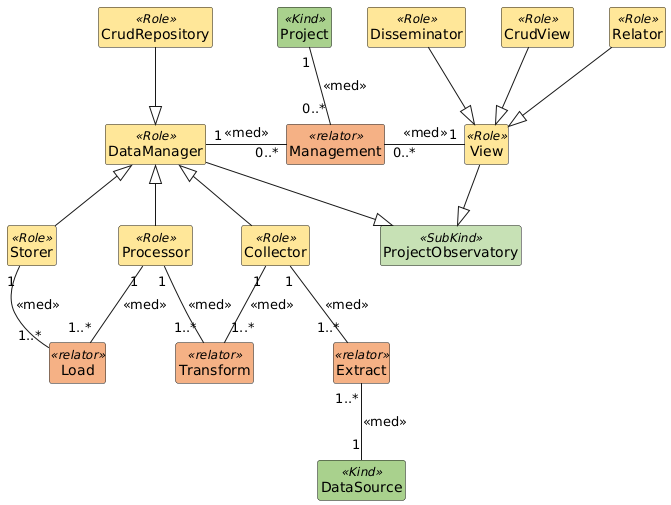
\includegraphics[width=1\linewidth]{imagens/mpo_structures_observatory_formalization.png}
    \caption{Formalização da organização de um observatório de acordo com o MPO. Fonte: Próprio autor.}
    \label{fig:mpo_class_tree}
\end{figure}

No diagrama, o \textit{ProjectObservatory} é modelado como um \textit{subkind} \cite{ontouml_readthedocs}, enquanto \textit{Project} e \textit{DataSource} são tratados como \textit{kinds} \cite{ontouml_readthedocs} do domínio. As classes \textit{View}, \textit{Disseminator}, \textit{Relator}, \textit{DataManager}, \textit{CrudManager}, \textit{Collector}, \textit{Processor} e \textit{Storer} são representadas como \textit{roles} \cite{ontouml_readthedocs}, refletindo papéis assumidos no contexto do observatório. As classes \textit{Management}, \textit{Extract}, \textit{Transform} e \textit{Load} são modeladas como \textit{relators}\cite{ontouml_readthedocs}, cuja existência é fundamentada pelas mediações estabelecidas com \textit{View}, \textit{DataManager}, \textit{Project} e \textit{DataSource}, representadas pelos estereótipos \textit{<<mediation>>}\cite{ontouml_readthedocs}(<<med>>). As generalizações presentes organizam especializações desses papéis, enquanto as sequências de mediação ilustram o fluxo ontológico das etapas de extração, transformação, carregamento e gerenciamento no observatório, preservando coerência estrutural entre os elementos modelados.

Na camada de agentes do MPO \cite{vieira2022thesis}, o diagrama a seguir tem como objetivo representar os atores que participam direta ou indiretamente do funcionamento do observatório. Essa camada evidencia quem são os sujeitos envolvidos, os papéis que desempenham e como suas ações contribuem para a dinâmica operacional do sistema. No diagrama, são modelados os elementos pertencentes às subcamadas atores e motivações, que organizam conceitualmente essa camada e permitem compreender tanto os agentes quanto as razões que orientam sua atuação.

\begin{figure}[H]
    \centering
    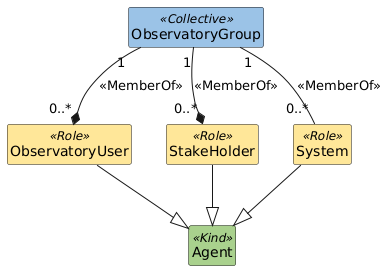
\includegraphics[width=0.75\linewidth]{imagens/mpo_agents_formalization.png}
    \caption{Formalização dos agentes de um observatório de acordo com o MPO. Fonte: Próprio autor.}
    \label{fig:mpo_class_tree}
\end{figure}

As classes \textit{ObservatoryUser}, \textit{StakeHolder} e \textit{System} são modeladas como \textit{roles} \cite{ontouml_readthedocs}, representando papéis contextuais assumidos por agentes conforme suas funções no observatório. A classe \textit{Agent} é modelada como um \textit{kind} \cite{ontouml_readthedocs}, caracterizando um tipo ontologicamente rígido que fornece a base para a especialização desses papéis. A classe \textit{ObservatoryGroup} é modelada como um \textit{collective} \cite{ontouml_readthedocs}, representando um grupo cujas partes possuem granularidade interna e são constituídas por múltiplos agentes desempenhando diferentes papéis. O estereótipo \textit{<<MemberOf>>} \cite{ontouml_readthedocs} é utilizado para representar relações de pertencimento em que indivíduos — aqui, \textit{ObservatoryUser}, \textit{StakeHolder} e \textit{System} — compõem estruturalmente o \textit{ObservatoryGroup}. Essas relações refletem a forma como conjuntos de agentes organizam-se em grupos dentro do domínio, preservando coerência com as restrições ontológicas estabelecidas pela UFO \cite{guizzardi2008grounding}.

Cabe destacar que, embora um sistema computacional externo possa existir
de forma independente do observatório e, sob esse aspecto, sugerir uma
classificação como \textit{kind}, a decisão de modelar \textit{System}
como \textit{role} decorre do recorte conceitual adotado nesta ontologia:
o que está sendo formalizado não é o sistema computacional em sua
existência autônoma, mas sim o papel relacional que esse sistema assume
\textit{quando integrado ao contexto do observatório}, isto é, quando
atua como fonte ou consumidor de dados, executor de processos ou
interface de acesso no âmbito da camada de Agentes. Essa classificação é
consistente com o tratamento dado às demais especializações de
\textit{Agent} (\textit{ObservatoryUser} e \textit{StakeHolder}), que
também representam papéis contextuais desempenhados por entidades cuja
existência independe da relação com o observatório --- uma pessoa existe
independentemente de ser usuária ou \textit{stakeholder} de um
observatório específico, da mesma forma que um sistema existe
independentemente de estar integrado a ele. O \textit{kind} subjacente ao
papel \textit{System}, ou seja, o tipo rígido que fundamenta sua
existência fora do contexto relacional do observatório, não foi
explicitado no diagrama, constituindo uma simplificação do modelo cuja
explicitação é apontada como melhoria para trabalhos futuros.

Por fim, apresenta-se o diagrama completo em OntoUML \cite{ontouml_readthedocs}, cujo objetivo é evidenciar a integração entre todas as camadas do MPO\cite{vieira2022thesis} e demonstrar como elas se articulam para representar o funcionamento do observatório como um todo. A visualização conjunta permite compreender de forma mais ampla como estruturas, agentes, e processos se conectam, revelando a lógica interna do modelo e o papel desempenhado por cada componente na dinâmica global do sistema.

\begin{figure}[H]
    \centering
    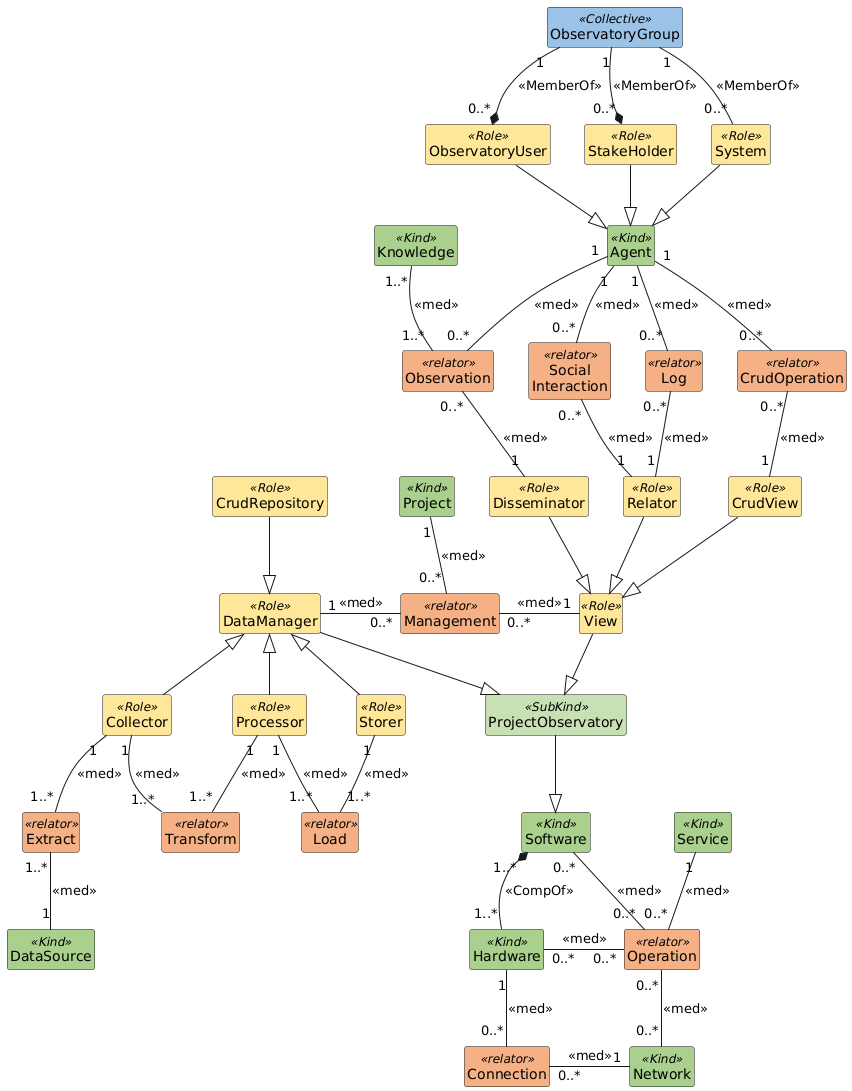
\includegraphics[width=1\linewidth]{imagens/mpo_formalization.png}
    \caption{Formalização do MPO. Fonte: Próprio autor.}
    \label{fig:mpo_class_tree}
\end{figure}

\section{Implementação}
A etapa de implementação, conforme definida pela \textit{Methontology}\cite{fernandez1997methontology}, corresponde à transposição do modelo ontológico previamente formalizado para um ambiente computacional, utilizando uma linguagem formal e uma ferramenta de suporte adequadas. Nessa fase, o objetivo central é tornar a ontologia operacional, permitindo sua validação sintática e semântica, bem como sua utilização em processos de inferência automática.

No contexto deste trabalho, a implementação representa uma evolução direta da etapa de formalização, na qual os conceitos, relações e restrições definidos conceitual e ontologicamente foram codificados na ferramenta Protégé, adotando-se a linguagem OWL. Essa transposição possibilitou verificar a consistência do modelo, explicitar axiomas formais e definir restrições que não são plenamente expressáveis nos modelos conceituais, mas que são essenciais para garantir precisão semântica e capacidade de inferência.

Os artefatos produzidos nessa etapa refletem, portanto, um nível mais elevado de formalismo em relação aos resultados apresentados anteriormente, mantendo total aderência às decisões ontológicas estabelecidas na formalização. Assim como realizado nas etapas anteriores, os resultados da implementação são apresentados de forma segmentada, com o intuito de facilitar o entendimento e a análise do leitor. Essa organização permite observar, de maneira gradual, como os elementos conceituais do modelo foram efetivamente materializados em uma ontologia computável.

A Figura \ref{fig:observatory_infra} apresenta a implementação da infraestrutura do observatório, conforme o MPO \cite{vieira2022thesis}, realizada por meio da ferramenta Protégé. Nessa representação, são contemplados os conceitos ontológicos relacionados aos recursos computacionais que sustentam o funcionamento do observatório de projetos. Essa dimensão da ontologia formaliza os elementos que constituem a base técnica necessária para a operação das demais dimensões do modelo. A representação evidencia a organização e as relações entre esses conceitos, assegurando uma estrutura semanticamente coerente e alinhada aos requisitos de interoperabilidade, escalabilidade e suporte às atividades de análise.

\begin{figure}[H]
    \centering
    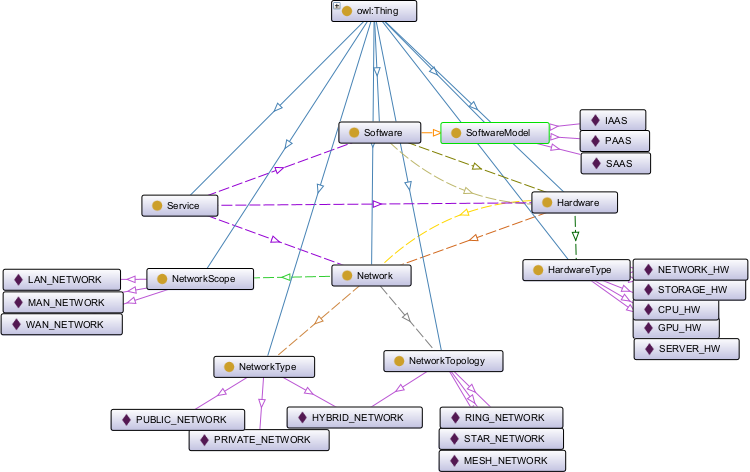
\includegraphics[width=1\linewidth]{imagens/observatory_infra.png}
    \caption{Implementação da infraestrutura de um observatório de acordo com o MPO. Fonte: Próprio autor.}
    \label{fig:observatory_infra}
\end{figure}

A Figura \ref{fig:observatory_organization} ilustra a organização do observatório, conforme o MPO \cite{vieira2022thesis}, implementada por meio da ferramenta Protégé, concentrando os conceitos ontológicos associados à sua estrutura interna, características, componentes e conteúdos. Essa dimensão da ontologia descreve como o observatório é concebido sob a perspectiva organizacional, explicitando os elementos que definem sua configuração, seus serviços e as formas de estruturação e disponibilização da informação. A segmentação dessa representação possibilita compreender, de maneira isolada, a lógica organizacional do observatório e o papel desempenhado por cada conceito no suporte às atividades de observação e transparência.

\begin{figure}[H]
    \centering
    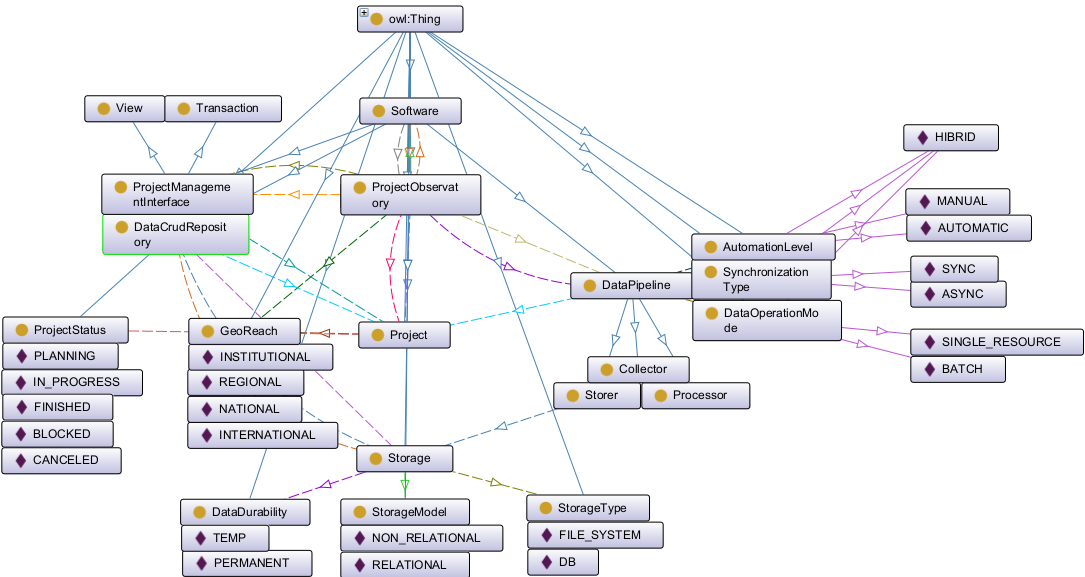
\includegraphics[width=1\linewidth]{imagens/observatory_organization.png}
    \caption{Implementação da organização de um observatório de acordo com o MPO. Fonte: Próprio autor.}
    \label{fig:observatory_organization}
\end{figure}

A Figura \ref{fig:mpo_class_tree} apresenta a dimensão de agentes do observatório, conforme o MPO \cite{vieira2022thesis}, implementada por meio da ferramenta Protégé, abrangendo os conceitos ontológicos relacionados aos atores envolvidos e às motivações que orientam suas interações com o sistema. Essa dimensão da ontologia formaliza os papéis desempenhados pelos diferentes tipos de agentes, bem como seus interesses, responsabilidades e formas de participação no observatório. A representação evidencia a relevância dos agentes como elementos centrais para o uso, a governança e a evolução do observatório, reforçando a dimensão socioorganizacional do modelo ontológico.

\begin{figure}[H]
    \centering
    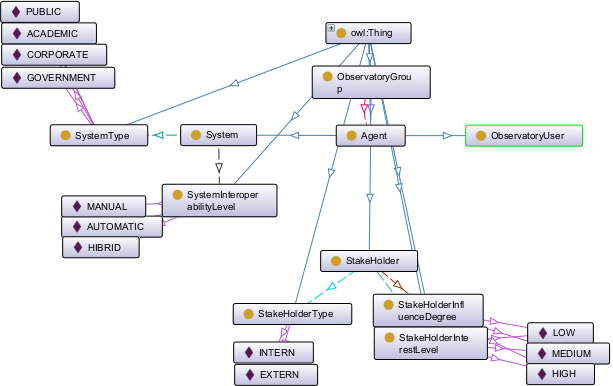
\includegraphics[width=1\linewidth]{imagens/observatory_agents.png}
    \caption{Implementação dos agentes de um observatório de acordo com o MPO. Fonte: Próprio autor.}
    \label{fig:mpo_class_tree}
\end{figure}

Por fim, a Figura \ref{fig:onto_mpo} apresenta a visão integrada da ontologia "OntoMPO", conforme o MPO \cite{vieira2022thesis}, implementada por meio da ferramenta Protégé, reunindo as dimensões de estruturas, processos e agentes em um único modelo ontológico coeso. Essa representação consolidada evidencia as relações estabelecidas entre os diferentes conjuntos de conceitos, possibilitando uma compreensão global da ontologia proposta. A visualização da ontologia completa demonstra como as dimensões previamente apresentadas se complementam e interagem, reforçando a consistência semântica do modelo e sua adequação para representar, de forma abrangente, o MPO \cite{vieira2022thesis}.

\begin{figure}[H]
    \centering
    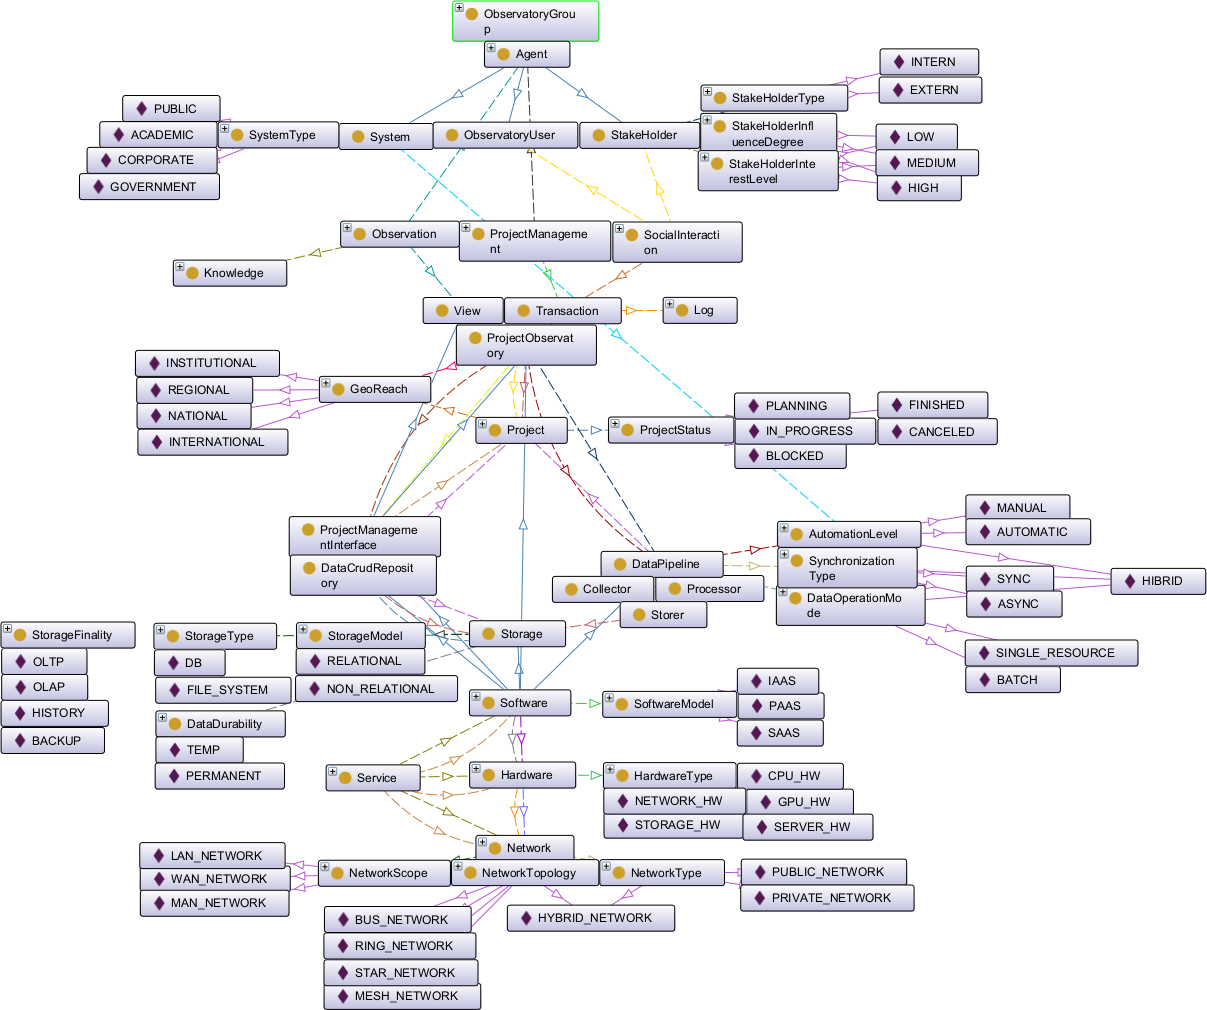
\includegraphics[width=1\linewidth]{imagens/onto_mpo.png}
    \caption{Implementação da OntoMPO. Fonte: Próprio autor.}
    \label{fig:onto_mpo}
\end{figure}

Como resultado da etapa de implementação, a ontologia foi analisada a partir de métricas estruturais extraídas por meio da ferramenta Protégé, com o objetivo de caracterizar seu tamanho, grau de detalhamento e complexidade lógica. A ontologia resultante é composta por \textbf{43 classes}, \textbf{45 propriedades de objeto}, \textbf{59 propriedades de dados} e \textbf{53 indivíduos}, refletindo a abrangência conceitual necessária para representar o domínio de observatórios de projetos. No que se refere à expressividade lógica, o modelo apresenta um total de \textbf{693 axiomas}, dos quais \textbf{434} correspondem a \textbf{axiomas lógicos} e \textbf{198} a \textbf{axiomas de declaração}, evidenciando um nível significativo de formalização semântica. Esses valores indicam que a ontologia ultrapassa uma estrutura meramente taxonômica, incorporando restrições, relações e definições formais que viabilizam inferência automática, mantendo, entretanto, um equilíbrio entre expressividade e complexidade computacional.

É importante destacar que o número de classes da OntoMPO (43) não
corresponde diretamente ao total de 61 conceitos originalmente
identificados no MPO~\cite{vieira2022thesis}. Essa diferença decorre do processo de
formalização ontológica, no qual nem todo conceito do modelo original foi
necessariamente representado como uma classe. Em particular, os termos
da subcamada \textit{Características} da camada Estruturas --- como
\textit{Sustentabilidade}, \textit{Abrangência}, \textit{Interoperabilidade},
\textit{Acesso} e \textit{Rede de Colaboração} --- correspondem, em sua
natureza, a propriedades e qualidades associadas às classes da camada
Estruturas, e não a entidades com identidade própria. Por essa razão,
durante a etapa de conceitualização, esses conceitos foram formalizados
como atributos das classes correspondentes, em vez de classes
independentes. A documentação detalhada do mapeamento entre os 61
conceitos do MPO e os elementos da OntoMPO (classes, propriedades ou
axiomas) constitui uma limitação deste trabalho, recomendando-se sua
sistematização como trabalho futuro por meio de uma tabela de
rastreabilidade conceito-a-elemento.

\begin{figure}[H]
    \centering
    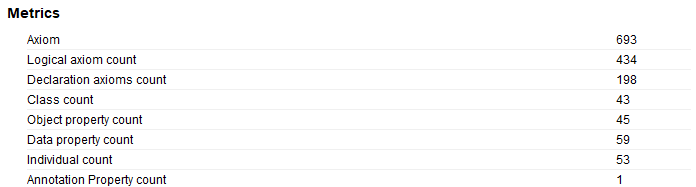
\includegraphics[width=1\linewidth]{imagens/onto_mpo_metrics.png}
    \caption{Métricas da OntoMPO. Fonte: Próprio autor.}
    \label{fig:mpo_class_tree}
\end{figure}

\section{Avaliação}

Esta seção apresenta a avaliação da ontologia desenvolvida para o MPO \cite{vieira2022thesis}. A avaliação teve como objetivo analisar a adequação conceitual, a coerência semântica e a consistência lógica do modelo ontológico, considerando o propósito estabelecido e as diretrizes metodológicas adotadas ao longo de seu desenvolvimento.

Em consonância com a abordagem proposta pela \textit{Methontology} \cite{fernandez1997methontology}, a avaliação concentrou-se na análise do artefato ontológico em si, contemplando aspectos conceituais e lógicos. Não foram conduzidos experimentos em ambientes operacionais nem exploradas capacidades de inferência automática, uma vez que o foco deste trabalho reside na formalização conceitual do domínio e na verificação da correção e consistência do modelo proposto.

A avaliação foi estruturada em duas abordagens complementares. A primeira corresponde à avaliação conceitual, voltada à análise da aderência da ontologia ao domínio dos observatórios de projetos. A segunda consiste na avaliação por meio de questões de competência, cujo objetivo é verificar se a ontologia é capaz de responder adequadamente a consultas representativas do domínio.

Dessa forma, os resultados apresentados a seguir buscam demonstrar que a ontologia representa de maneira fiel os conceitos centrais do MPO, apresenta consistência lógica e dispõe de uma estrutura formal adequada para suportar análises conceituais e consultas baseadas em questões de competência.

A avaliação do OntoMPO foi
conduzido por meio de análise conceitual e verificação de questões de competência baseadas em SPARQL, sem
sessões de validação estruturadas envolvendo especialistas no domínio, o que fortaleceria ainda mais a confiança em
a cobertura e adequação semântica da ontologia. Além disso, dada a natureza conceitual do OntoMPO -
focado na formalização de domínio em vez de implantação operacional - recursos de inferência automatizados
não foram explorados em profundidade. A ontologia foi projetada para representar formalmente o conceito conceitual do MPO
estrutura e sua expressividade atual em OWL 2 DL, embora suficiente para consulta semântica e
verificação de consistência, não foi estendido para apoiar raciocínio complexo baseado em regras ou inferência de cadeia de funções.

\subsection{Avaliação conceitual}

A avaliação conceitual da ontologia teve como objetivo verificar sua adequação em relação ao domínio dos observatórios de projetos, conforme definido pelo MPO \cite{vieira2022thesis}. Essa avaliação concentrou-se na análise da cobertura conceitual, da coerência semântica e da correspondência entre os conceitos do modelo de referência e os elementos formalizados na ontologia, incluindo classes, propriedades e restrições.

Observou-se que os principais elementos conceituais do MPO \cite{vieira2022thesis}, tais como agentes, processos e estruturas, encontram correspondência explícita na ontologia, preservando a semântica originalmente proposta no modelo conceitual. A organização das classes reflete a decomposição do domínio apresentada no MPO, permitindo distinguir de forma clara entidades, relações e atributos relevantes ao funcionamento de um observatório de projetos.

Adicionalmente, a definição das propriedades e restrições ontológicas contribuiu para explicitar relações semânticas entre os conceitos, como a participação de agentes em processos e a associação entre estruturas organizacionais e os conteúdos por elas produzidos. A utilização de enumerações para representar conjuntos finitos de valores mostrou-se adequada ao domínio, uma vez que tais elementos representam categorias de classificação e não entidades do mundo real.

De modo geral, a ontologia apresenta aderência conceitual ao MPO, oferecendo uma representação formal consistente e semanticamente clara do domínio dos observatórios de projetos.

\subsection{Avaliação por questões de competência}

A avaliação por questões de competência foi conduzida com o objetivo de verificar a capacidade da ontologia em responder a consultas representativas do domínio previamente definidas na etapa de especificação. Essas questões orientam o desenvolvimento e a validação da ontologia, permitindo avaliar se o modelo formal é capaz de representar adequadamente os conhecimentos relevantes do domínio.

Para responder às questões de competência, foram realizadas consultas SPARQL sobre a ontologia implementada. Essas consultas permitiram extrair informações relativas à organização hierárquica das classes e às relações semânticas estabelecidas entre os conceitos.

Os resultados das consultas foram posteriormente processados por meio de um script em Python, responsável por organizar as classes em estruturas hierárquicas e identificar as relações semânticas entre os conceitos com base nas propriedades definidas na ontologia.

\subsubsection{QC1 – Como os conceitos da ontologia estão organizados hierarquicamente?}

A questão de competência QC1 tem como objetivo identificar a organização hierárquica geral dos conceitos presentes na ontologia. Para responder a essa questão, foi utilizada uma consulta SPARQL responsável por recuperar as relações de especialização entre as classes da ontologia por meio da propriedade \textit{rdfs:subClassOf}.

\begin{figure}[H]
\centering
\begin{minipage}{0.7\linewidth}
\begin{verbatim}
SELECT ?class ?superclass
WHERE {
    ?class rdfs:subClassOf ?superclass .
}
\end{verbatim}
\end{minipage}
\caption{Consulta SPARQL utilizada para verificar a ontologia hierarquicamente. Fonte: Próprio autor.}
\label{fig:avaliacao_sparql_qc1}
\end{figure}

Os resultados da consulta foram processados por meio de um script em Python, cuja lógica pode ser descrita conforme o pseudo-código a seguir.

\begin{figure}[H]
\centering
\begin{minipage}{0.7\linewidth}
\begin{verbatim}
For each class returned by the query:
    Identify its superclass
    Create hierarchical relation (class -> superclass)

Construct hierarchical tree of ontology concepts
\end{verbatim}
\end{minipage}
\caption{Consulta SPARQL utilizada para verificar a ontologia hierarquicamente. Fonte: Próprio autor.}
\label{fig:avaliacao_script_qc1}
\end{figure}

A análise evidenciou que a ontologia apresenta uma estrutura hierárquica bem definida, na qual conceitos mais gerais são progressivamente especializados em subclasses mais específicas.

\subsubsection{QC2 – Como a camada de estruturas é representada na ontologia?}

A questão QC2 busca identificar como os conceitos associados à camada de estruturas do modelo MPO estão organizados na ontologia. Para essa análise, foi considerada como classe raiz o conceito \textit{Software}, a partir do qual foram identificadas as subclasses e relações semânticas associadas. A mesma consulta utilizada na QC1 foi aplicada considerando apenas as classes pertencentes à hierarquia da classe raiz analisada. Os resultados foram organizados pelo script de processamento, permitindo visualizar a estrutura hierárquica da camada de estruturas.

\begin{figure}[H]
\centering
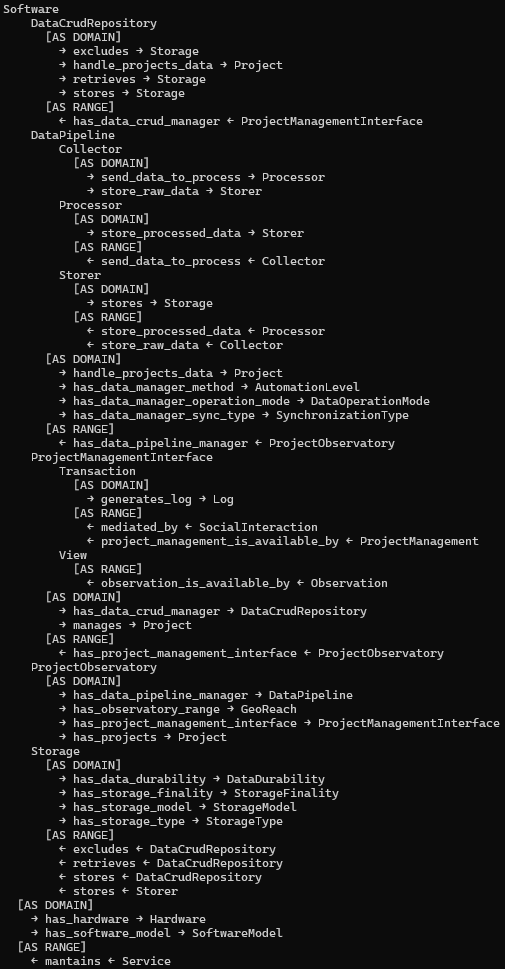
\includegraphics[width=0.8\linewidth]{avaliacao_4.png}
\caption{Exemplo de resultado da análise hierárquica e semântica da camada Estruturas. Fonte: Próprio autor}
\label{fig:resultado_estrutura}
\end{figure}

Os resultados demonstram que a camada de estruturas apresenta uma organização hierárquica coerente, com subclasses especializadas que representam diferentes componentes da infraestrutura e organização do observatório.

\subsubsection{QC3 – Como a camada de processos é representada na ontologia?}

A questão QC3 analisa a representação da camada de processos na ontologia. Para essa análise foi considerada a classe raiz \textit{ProjectManagement}. A partir dela foram identificadas as subclasses associadas e as relações semânticas que conectam os processos aos demais conceitos da ontologia.

\begin{figure}[H]
\centering
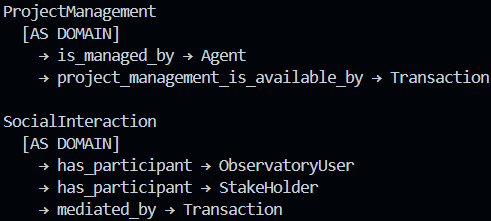
\includegraphics[width=0.6\linewidth]{avaliacao_4.1.png}
\caption{Exemplo de resultado da análise hierárquica e semântica da camada Processos. Fonte: Próprio autor}
\label{fig:resultado_processos}
\end{figure}

A análise evidenciou que os processos estão organizados em uma estrutura hierárquica clara, representando diferentes atividades relacionadas ao funcionamento de um observatório de projetos.

\subsubsection{QC4 – Como a camada de agentes é representada na ontologia?}

A questão QC4 investiga a forma como os agentes envolvidos no domínio são representados na ontologia. Para essa análise foi considerada a classe raiz \textit{Agent}, a partir da qual foram identificadas as subclasses correspondentes aos diferentes tipos de atores envolvidos no domínio.

\begin{figure}[H]
\centering
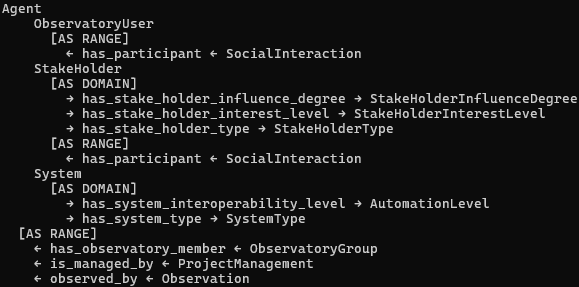
\includegraphics[width=0.6\linewidth]{avaliacao_5.png}
\caption{Exemplo de resultado da análise hierárquica e semântica da camada Agentes. Fonte: Próprio autor}
\label{fig:resultado_agentes}
\end{figure}

Os resultados demonstram que os diferentes tipos de agentes estão organizados em uma hierarquia consistente, permitindo distinguir papéis e categorias de atores presentes no domínio dos observatórios de projetos.

\subsubsection{QC5 – Quais são as relações existentes entre estruturas, processos e agentes?}

A questão de competência QC5 tem como objetivo identificar as relações semânticas existentes entre as diferentes camadas da ontologia. Para isso, foram utilizadas consultas SPARQL voltadas à extração de propriedades do tipo \textit{owl:ObjectProperty}, considerando seus domínios e alcances.

\begin{figure}[H]
\centering
\begin{minipage}{0.7\linewidth}
\begin{verbatim}
SELECT ?property ?domain ?range
WHERE {
    ?property rdf:type owl:ObjectProperty .
    ?property rdfs:domain ?domain .
    ?property rdfs:range ?range .
}
\end{verbatim}
\end{minipage}
\caption{Consulta SPARQL utilizada para verificar as propriedades de objetos, considerando seus domínios e alcances. Fonte: Próprio autor.}
\label{fig:avaliacao_script_qc1}
\end{figure}

A análise dos resultados demonstrou que as conexões entre estruturas, processos e agentes são frequentemente mediadas por conceitos centrais da ontologia, como \textit{Observation} e \textit{Knowledge}. Esses conceitos atuam como pontos de integração entre diferentes partes do modelo, permitindo articular as informações produzidas e utilizadas no contexto dos observatórios de projetos.

\begin{figure}[H]
\centering
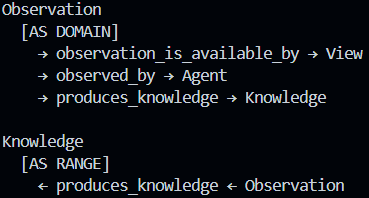
\includegraphics[width=0.5\linewidth]{image.png}
\caption{Exemplo de resultado da análise das relações entre camadas. Fonte: Próprio autor}
\label{fig:resultado_intercamadas}
\end{figure}

Dessa forma, observa-se que as diferentes camadas do modelo MPO não se conectam apenas por relações diretas, mas também por meio de mecanismos de mediação semântica, garantindo maior coesão e modularidade na estrutura da ontologia.

\subsection{OntoMPO}

Como principal resultado desta pesquisa, foi desenvolvida a \textit{OntoMPO}, uma ontologia de domínio destinada à formalização semântica do Modelo para Observatórios de Projetos (MPO) \cite{vieira2022thesis}. A OntoMPO explicita de maneira formal os conceitos, relações e restrições presentes no modelo conceitual original, permitindo sua representação computacional e ampliando suas possibilidades de aplicação em ambientes informacionais e analíticos.

A ontologia foi construída seguindo as etapas da metodologia \textit{Methontology} \cite{fernandez1997methontology}, contemplando as fases de especificação, conceitualização, formalização, integração, implementação e avaliação. Durante o processo de modelagem conceitual, foi utilizada a linguagem OntoUML \cite{ontouml_readthedocs}, que fornece suporte à representação de categorias ontológicas fundamentadas na Unified Foundational Ontology (UFO), garantindo maior rigor semântico na definição dos elementos do domínio.

A OntoMPO estrutura os conceitos do domínio de observatórios de projetos com base nas dimensões fundamentais definidas pelo MPO, especialmente Estruturas, Processos e Agentes, estabelecendo relações semânticas entre esses elementos e organizando-os em uma hierarquia conceitual coerente. Essa estrutura permite representar de forma explícita os papéis desempenhados pelos agentes, os processos envolvidos na produção e disseminação de informações e os elementos estruturais que compõem os observatórios de projetos.

A implementação da OntoMPO foi realizada na linguagem OWL, padrão amplamente utilizado para a representação de ontologias na Web Semântica. Essa implementação possibilita que a ontologia seja processada por ferramentas computacionais, permitindo a realização de consultas semânticas, inferências automáticas e integração com outros sistemas baseados em tecnologias semânticas.

Como resultado, a OntoMPO fornece uma base conceitual formal que reduz ambiguidades presentes na descrição original do MPO e estabelece um vocabulário estruturado para o domínio de observatórios de projetos. Essa formalização contribui para a padronização conceitual do domínio e cria condições para o desenvolvimento de aplicações futuras, tais como sistemas de apoio à gestão de observatórios, plataformas de compartilhamento de conhecimento e mecanismos de análise comparativa entre diferentes observatórios.

A descrição completa da ontologia, incluindo suas classes, propriedades e axiomas principais, é apresentada no Apêndice desta dissertação.
